% =============================================================================
%  Prediction Markets Dashboard -- Technical Submission Report
%  Build:  tectonic report.tex
% =============================================================================
\documentclass[11pt,a4paper]{article}

\usepackage[T1]{fontenc}
\usepackage{amsmath}
\usepackage{XCharter}
\usepackage[charter,scaled=1.04]{newtxmath}
\usepackage[varqu,scaled=0.96]{zi4}
\usepackage[margin=2.5cm,top=2.4cm,bottom=2.4cm]{geometry}
\usepackage[skip=7pt plus 2pt, indent=0pt]{parskip}
\usepackage{graphicx}
\usepackage{booktabs}
\usepackage{tabularx}
\usepackage{xcolor}
\usepackage{titlesec}
\usepackage{enumitem}
\usepackage{listings}
\usepackage{tcolorbox}
\usepackage{tikz}
\usepackage{caption}
\usepackage{float}
\usepackage[section]{placeins}
\usepackage[hidelinks]{hyperref}

\usetikzlibrary{positioning,arrows.meta,fit,backgrounds}
\tcbuselibrary{skins,breakable}

\linespread{1.05}\selectfont

\makeatletter
\setlength{\@fptop}{0pt}
\renewcommand{\topfraction}{0.92}
\renewcommand{\textfraction}{0.08}
\renewcommand{\floatpagefraction}{0.75}
\makeatother

% ---------------------------------------------------------------- palette ---
\definecolor{poly}{HTML}{2F6FD0}
\definecolor{kalshi}{HTML}{0E8F72}
\definecolor{ink}{HTML}{1A1D23}
\definecolor{slate}{HTML}{5A6472}
\definecolor{rule}{HTML}{D6DAE0}
\definecolor{panel}{HTML}{F5F7F9}
\definecolor{amber}{HTML}{9A6700}
\definecolor{danger}{HTML}{B3261E}

\hypersetup{colorlinks=true,linkcolor=poly,urlcolor=poly}

% --------------------------------------------------------------- headings ---
\titleformat{\section}{\large\bfseries\color{ink}}{\thesection}{0.6em}{}
\titleformat{\subsection}{\normalsize\bfseries\color{ink}}{\thesubsection}{0.5em}{}
\titlespacing*{\section}{0pt}{1.6em}{0.6em}
\titlespacing*{\subsection}{0pt}{1.1em}{0.4em}

\captionsetup{font=small,labelfont={bf,color=slate},textfont={color=slate},labelsep=period}
\setlist{itemsep=3pt,parsep=0pt,topsep=4pt}
\renewcommand{\arraystretch}{1.2}

% --------------------------------------------------------------- listings ---
\lstdefinestyle{code}{
  basicstyle=\ttfamily\scriptsize,
  backgroundcolor=\color{panel},
  frame=leftline, framerule=1.6pt, rulecolor=\color{rule},
  xleftmargin=9pt, framexleftmargin=9pt,
  breaklines=true, showstringspaces=false,
  columns=fullflexible, keepspaces=true,
  aboveskip=9pt, belowskip=7pt,
}
\lstset{style=code}

\newtcolorbox{keybox}[1][]{
  enhanced, breakable, colback=panel, colframe=poly,
  boxrule=0pt, leftrule=2.5pt, arc=1pt,
  left=9pt,right=9pt,top=7pt,bottom=7pt, #1
}

\newcommand{\code}[1]{{\ttfamily\small #1}}
\newcommand{\file}[1]{{\ttfamily\small\color{slate} #1}}
\newcommand{\PM}{{\color{poly}\textbf{Polymarket}}}
\newcommand{\KS}{{\color{kalshi}\textbf{Kalshi}}}

% =============================================================================
\begin{document}

\begin{center}
{\LARGE\bfseries\color{ink} Prediction Markets Dashboard\par}
\vspace{0.35em}
{\large\color{slate} Cross-Exchange Analytics for \textcolor{poly}{Polymarket} $\times$ \textcolor{kalshi}{Kalshi}\par}
\vspace{0.7em}
{\normalsize Nikhil Pothuganti \;$\cdot$\; \today\par}
\vspace{0.35em}
{\small\color{slate} Next.js 15 $\cdot$ TypeScript $\cdot$ 6{,}372 LOC $\cdot$ 3 routes $\cdot$ 11 API endpoints\par}
\vspace{0.5em}
\textcolor{rule}{\rule{0.9\textwidth}{0.8pt}}
\end{center}

% =============================================================================
\section{The Problem}

Prediction markets are fragmented. The same question --- who wins the 2028 US election, who
lifts the 2026 World Cup --- trades on both \PM{} and \KS{}, at different prices, under
different resolution rules.

A gap between the two venues looks like free money. It usually isn't.

This dashboard pulls live order books and price history from both venues, works out which
markets are the same question, then tests every gap three ways:

\begin{itemize}
  \item \textbf{Is it fillable?} Walk both books. Don't quote the touch.
  \item \textbf{Does it survive fees and time?} \KS{}'s fee is non-linear, and capital is
        locked until the market resolves.
  \item \textbf{Do the two markets actually pay the same?} Often they don't.
\end{itemize}

\begin{keybox}
\textbf{Thesis.} A visible price gap is by default \textbf{not} an edge. A spread is shown as
tradeable only when the match is \textsc{verified}, the depth- and fee-aware edge is positive,
and the divergence assessment sits beside it.

\smallskip
\textbf{Result.} On the 2028 President market, an apparent 8-point gap is really about
\textbf{0.8\%/year}. A T-bill beats it. And the venues don't settle on the same event --- \KS{}
pays on who is \emph{inaugurated}, \PM{} on the \emph{AP/Fox/NBC race call}. It was never a
lock.
\end{keybox}

That thesis drives everything: why the matcher rejects rather than guesses, why the engine
walks the book, why returns are annualised, why the divergence layer exists.

\begin{figure}[htbp]
\centering
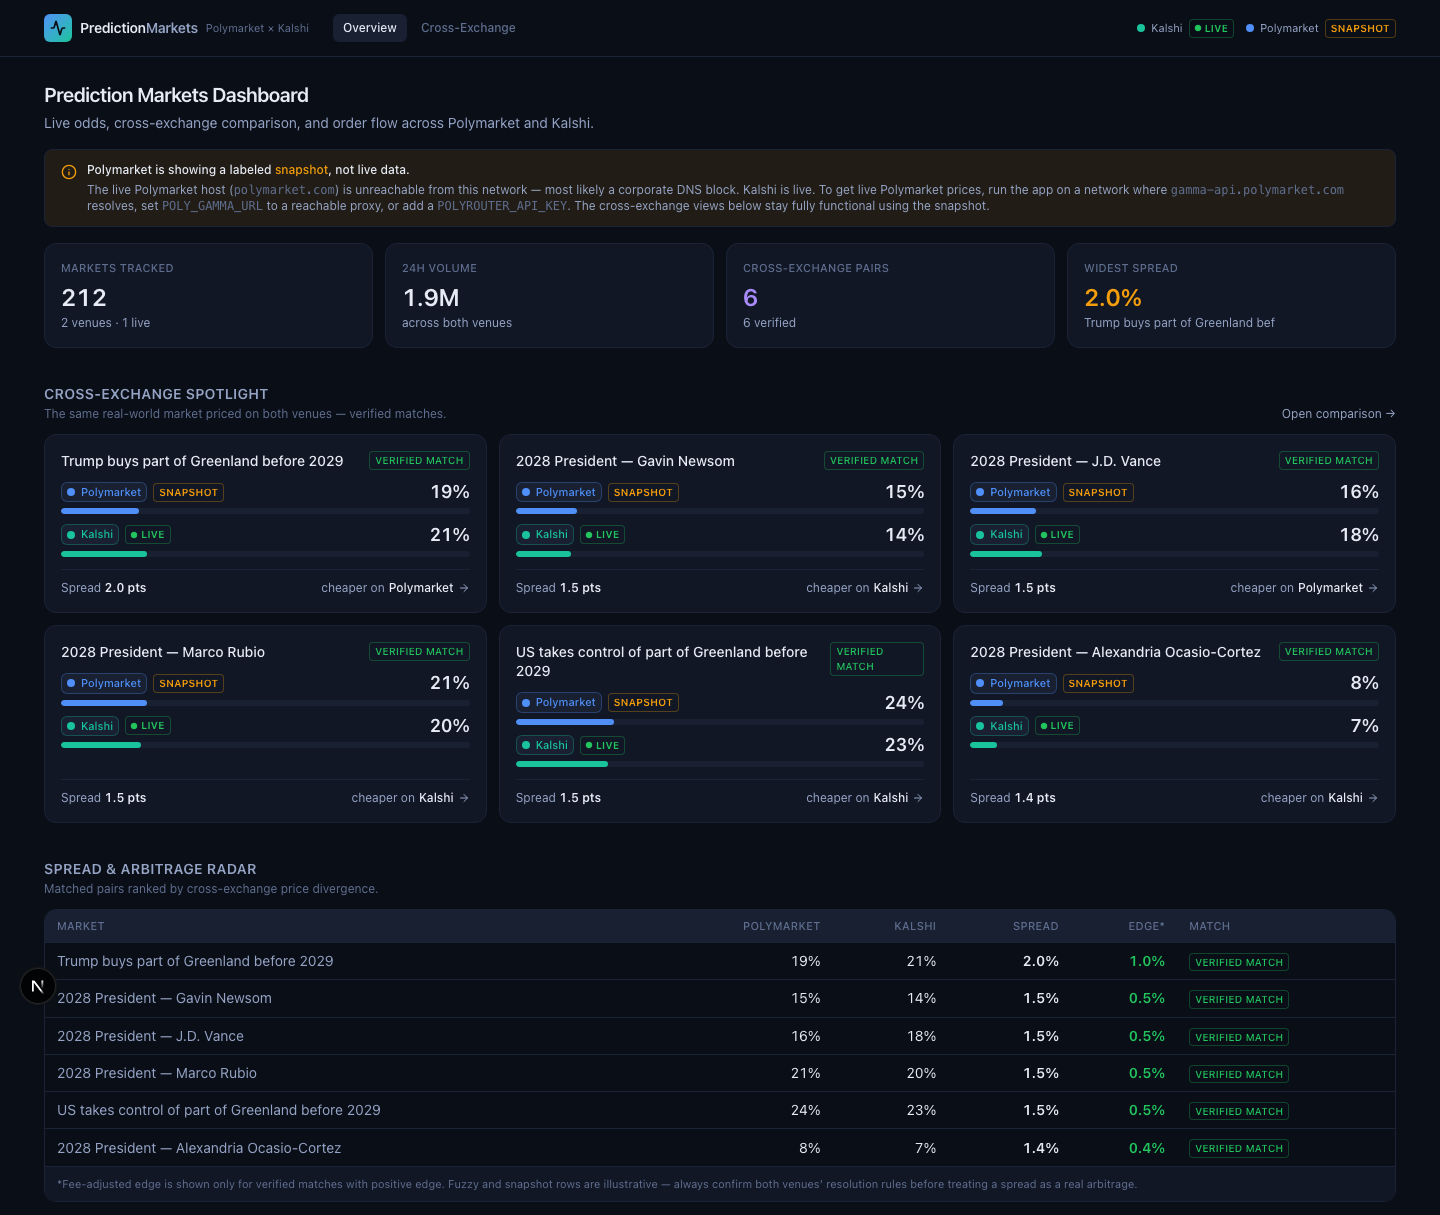
\includegraphics[width=\textwidth]{figures/overview-analytics.png}
\caption{Overview. Badges top-right show \KS{} \textsc{live} and \PM{} in labeled
\textsc{snapshot} mode (\S\ref{sec:eng}). Below: corpus stats, verified pairs, and the
arbitrage radar ranked by divergence.}
\label{fig:overview}
\end{figure}

% =============================================================================
\section{Architecture}

One Next.js 15 App Router deployment. No separate backend --- the server tier is route
handlers under \file{app/api/}, and they are the only thing that talks to a venue.

That isn't stylistic. \KS{} returns \code{403} to any request carrying an \code{Origin}
header, so a browser fetch cannot work. Proxying server-side also puts normalisation, caching
and degradation in one place.

\begin{figure}[htbp]
\centering
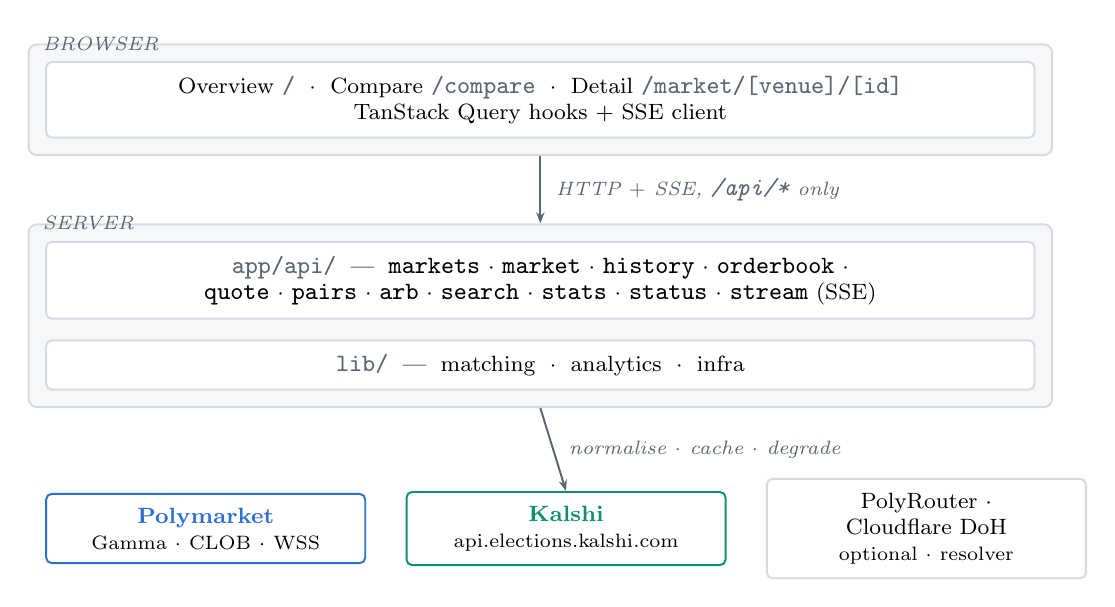
\begin{tikzpicture}[
  font=\footnotesize, node distance=0pt,
  box/.style={draw=rule,line width=0.7pt,rounded corners=2pt,align=center,
              inner sep=5pt,fill=white,text width=12.2cm},
  sbox/.style={draw=rule,line width=0.7pt,rounded corners=2pt,align=center,
               inner sep=5pt,fill=white,text width=3.7cm},
  lay/.style={draw=rule,line width=0.7pt,rounded corners=3pt,fill=panel,inner sep=6pt},
  ar/.style={-{Stealth[length=4pt]},draw=slate,line width=0.7pt},
  lbl/.style={font=\scriptsize\itshape,color=slate},
]
\node[box] (br)
  {Overview \mbox{\file{/}} \;$\cdot$\; Compare \mbox{\file{/compare}} \;$\cdot$\;
   Detail \mbox{\file{/market/[venue]/[id]}}\\
   TanStack Query hooks $+$ SSE client};
\begin{scope}[on background layer]
  \node[lay,fit=(br),label={[lbl,anchor=west,xshift=2pt]north west:BROWSER}] (brl) {};
\end{scope}

\node[box,below=13mm of br] (api)
  {\file{app/api/} \;---\; \code{markets} $\cdot$ \code{market} $\cdot$ \code{history} $\cdot$
   \code{orderbook} $\cdot$ \code{quote} $\cdot$ \code{pairs} $\cdot$ \code{arb} $\cdot$
   \code{search} $\cdot$ \code{stats} $\cdot$ \code{status} $\cdot$ \code{stream} (SSE)};
\node[box,below=2.5mm of api] (dom)
  {\file{lib/} \;---\; matching \;$\cdot$\; analytics \;$\cdot$\; infra};
\begin{scope}[on background layer]
  \node[lay,fit=(api)(dom),
        label={[lbl,anchor=west,xshift=2pt]north west:SERVER}] (srv) {};
\end{scope}

\node[sbox,below=13mm of dom.south west,anchor=north west,draw=poly] (upP)
  {\textcolor{poly}{\textbf{Polymarket}}\\{\scriptsize Gamma $\cdot$ CLOB $\cdot$ WSS}};
\node[sbox,right=5mm of upP,draw=kalshi] (upK)
  {\textcolor{kalshi}{\textbf{Kalshi}}\\{\scriptsize api.elections.kalshi.com}};
\node[sbox,right=5mm of upK] (upF)
  {PolyRouter $\cdot$ Cloudflare DoH\\{\scriptsize optional $\cdot$ resolver}};

\draw[ar] (brl.south) -- node[lbl,right=2pt]{HTTP $+$ SSE, \code{/api/*} only} (srv.north);
\draw[ar] (srv.south) -- node[lbl,right=2pt]{normalise $\cdot$ cache $\cdot$ degrade} (upK.north);
\end{tikzpicture}
\caption{Request topology. Caches are prewarmed at boot, so the first request doesn't pay the
$\sim$17\,s cold build. Most of the code is in \file{lib/} (3{,}297 LOC) rather than
\file{components/} (2{,}342) --- a data pipeline with a UI, not the reverse.}
\label{fig:arch}
\end{figure}

\begin{table}[htbp]
\centering\small
\begin{tabularx}{\textwidth}{@{}p{4.2cm}X@{}}
\toprule
\textbf{Feature} & \textbf{Summary} \\
\midrule
Cross-exchange comparison & Same question on both venues: dual-line history, live spread, both
  books, resolution rules side by side \\
Depth-aware arbitrage & Walks both books until the edge collapses; reports fillable size, net
  profit, annualised ROI \\
Resolution divergence & Flags matched pairs that would settle differently \\
Three-tier matching & Entity alignment, curated seed, IDF-weighted fuzzy fallback \\
Real-time order book & \PM{} over WebSocket $\rightarrow$ SSE; \KS{} polls at 2\,s \\
Arbitrage radar & Matched pairs ranked by divergence, filterable by category \\
Market browser & Both venues, server-side sort and filter, debounced search, infinite scroll \\
DNS-over-HTTPS & Live \PM{} data on networks that DNS-block it. No VPN \\
Per-venue degradation & \textsc{live}/\textsc{snapshot}/\textsc{offline}, labeled everywhere \\
Performance & Five SWR cache layers, boot prewarm, incremental chart updates \\
\bottomrule
\end{tabularx}
\caption{Feature summary. The three that distinguish this from a spread scanner are covered in
\S\ref{sec:match}--\ref{sec:div}.}
\end{table}

% =============================================================================
\section{Matching}
\label{sec:match}

The hardest part. There is no shared identifier between venues, so the join is inferred from
text --- and a false positive is worse than a miss, because it invents a spread between two
questions that aren't the same.

Three tiers run in order, each consuming markets from a shared pool.

\begin{table}[htbp]
\centering\small
\begin{tabularx}{\textwidth}{@{}p{1.3cm}p{2.8cm}Xp{1.7cm}@{}}
\toprule
\textbf{Tier} & \textbf{Method} & \textbf{How} & \textbf{Confidence} \\
\midrule
0 & Entity alignment & A registry maps a \PM{} event to a \KS{} series; every outcome aligns by
  canonical entity. 6 events, $\sim$108 sports pairs. & \textsc{verified} \\
1 & Curated seed & 6 hand-verified pairs, carrying both a live and a snapshot id. & \textsc{verified} \\
2 & IDF-weighted fuzzy & Weighted token overlap behind four guards, threshold $0.6$. & \textsc{fuzzy} \\
\bottomrule
\end{tabularx}
\caption{Confidence degrades down the stack. Only \textsc{verified} pairs can be presented as
arbitrage.}
\end{table}

\textbf{Tier 0} exists because text matching under-performs on a categorical event --- it only
``sees'' the candidates whose titles happen to look alike. Declaring the correspondence at the
\emph{event} level instead means the whole field pairs. Adding a league is one registry entry;
teams align by token overlap, so no roster data is needed. An alias table keeps \emph{Donald
Trump Jr} distinct from \emph{Donald Trump} --- exactly the collision that would otherwise
invent a huge spread.

\textbf{Tier 2} scores weighted token overlap. With $T(m)$ the token set of market $m$ after
stopwords, stemming and alias expansion, over $N$ documents:

\begin{equation}
\mathrm{idf}(t) = \log\!\left(1 + \frac{N}{\mathrm{df}(t)}\right),
\qquad
S(p,k) = \frac{\sum_{t \in T(p) \cap T(k)} \mathrm{idf}(t)}
              {\min\bigl(W(p), W(k)\bigr)},
\qquad
W(m) = \!\!\sum_{t \in T(m)}\!\! \mathrm{idf}(t) .
\end{equation}

Accept only if $S \geq 0.6$, at least 2 tokens are shared, and at least one shared token has
$\mathrm{df}(t) \leq 8$.

That last condition is what makes the tier usable. Every 2028 candidate shares \code{2028},
\code{president}, \code{nominee} --- without a rarity requirement they all match each other.
Requiring a rare token forces the match to rest on a name.

Four guards reject a candidate before scoring. Two were added to kill specific bad matches
found in testing:

\begin{itemize}
  \item \textbf{Question kind} --- \emph{nominee} / \emph{run} / \emph{winner} / \emph{host}
        never cross-match. This keeps ``will X \emph{win} the World Cup'' apart from ``will X
        \emph{host} it'': same entity, near-identical tokens, very different prices.
  \item \textbf{Multi-entity} --- a combined ``A, B or C'' market never matches a single-entity
        one.
  \item \textbf{Numbers} --- conflicting numerals separate ``$\geq$25bps'' from ``50bps''.
  \item \textbf{Category} --- must be equal.
\end{itemize}

After scoring, one more check: a fuzzy pair with spread $> 0.35$ is dropped. Two equivalent
liquid markets don't disagree by 35 points, so that gap is almost certainly a title collision.

% =============================================================================
\section{Arbitrage}
\label{sec:arb}

Differencing mid-prices gives an edge you cannot transact. You buy at the ask and sell at the
bid, and size at the touch is usually trivial.

On a binary market, \textsc{yes} on one venue plus \textsc{no} on the other redeems for exactly
\$1. Buying \textsc{no} at $1-b$ equals selling \textsc{yes} at bid $b$. So for a share bought
at ask $a$ and hedged at bid $b$:

\begin{equation}
\text{net edge/share} = b - a - \phi_{\text{buy}}(a) - \phi_{\text{sell}}(1-b),
\qquad
\text{capital/share} = a + (1-b),
\end{equation}

with $\phi_{\text{kalshi}}(p) = 0.07\,p\,(1-p)$ and $\phi_{\text{polymarket}}(p) = 0$. Note the
shape: \KS{}'s fee peaks at $p = 0.5$, so a flat fee assumption would misprice exactly the
mid-probability markets where spreads are widest.

The engine walks both ladders with two pointers --- asks ascending against bids descending,
consuming the smaller side each step, halting when the fee-adjusted edge goes non-positive.
Both directions are tried; the better wins.

\begin{figure}[htbp]
\centering
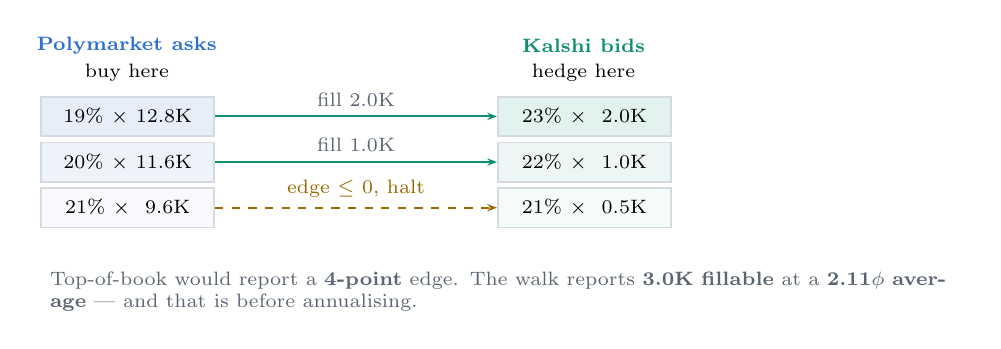
\begin{tikzpicture}[font=\scriptsize,
  lvl/.style={draw=rule,line width=0.6pt,minimum width=2.2cm,minimum height=5mm,anchor=west,align=center},
  hdr/.style={font=\scriptsize\bfseries,align=center},
  ar/.style={-{Stealth[length=3.5pt]},line width=0.7pt},
]
\node[hdr,color=poly] at (1.1,0.9) {Polymarket asks};
\node[hdr] at (1.1,0.55) {\normalfont buy here};
\node[hdr,color=kalshi] at (6.9,0.9) {Kalshi bids};
\node[hdr] at (6.9,0.55) {\normalfont hedge here};

\node[lvl,fill=poly!12] at (0,0)     (a1) {19\% $\times$ 12.8K};
\node[lvl,fill=poly!8]  at (0,-0.58) (a2) {20\% $\times$ 11.6K};
\node[lvl,fill=poly!4]  at (0,-1.16) (a3) {21\% $\times$ \ 9.6K};

\node[lvl,fill=kalshi!12] at (5.8,0)     (b1) {23\% $\times$ \ 2.0K};
\node[lvl,fill=kalshi!8]  at (5.8,-0.58) (b2) {22\% $\times$ \ 1.0K};
\node[lvl,fill=kalshi!4]  at (5.8,-1.16) (b3) {21\% $\times$ \ 0.5K};

\draw[ar,draw=kalshi] (a1.east) -- node[above,color=slate]{fill 2.0K} (b1.west);
\draw[ar,draw=kalshi] (a2.east) -- node[above,color=slate]{fill 1.0K} (b2.west);
\draw[ar,draw=amber,dashed] (a3.east) -- node[above,color=amber]{edge $\leq$ 0, halt} (b3.west);

\node[align=left,text width=11.6cm,color=slate,anchor=north west] at (0,-1.85)
  {Top-of-book would report a \textbf{4-point} edge. The walk reports \textbf{3.0K fillable} at
   a \textbf{2.11$\phi$ average} --- and that is before annualising.};
\end{tikzpicture}
\caption{The book walk (illustrative sizes). The reported edge averages over filled size, not
the touch.}
\label{fig:walk}
\end{figure}

\subsection{Annualisation --- the decisive step}

A cross-exchange lock is not a free roll. Capital sits committed until resolution, and for the
2028 market that is over two years.

\begin{equation}
\mathrm{ROI} = \frac{\text{net profit}}{\text{capital}},
\qquad
\mathrm{ROI}_{\text{ann}} = \frac{\mathrm{ROI}}{\tau},
\qquad
\tau = \frac{t_{\text{close}} - t_{\text{now}}}{365.25\ \text{days}} .
\end{equation}

Reported only when $\tau > 0.02$ years, below which annualising produces nonsense multipliers.
Benchmarked against a configurable risk-free rate (6\%/yr default): green when it clears,
amber when a Treasury bill beats it.

This is the most important number in the product. It turns the 8-point gap of \S1 into
0.8\%/year --- and shows it in amber.

\textbf{Two spread notions, on purpose.} \file{lib/match.ts} computes a naive
$|p_{\text{poly}} - p_{\text{kalshi}}|$ with a flat 1\% buffer: a cheap ranking pre-filter that
runs corpus-wide and needs no order book. \file{lib/arb.ts} does the real walk: the decision
number. So the radar ranks by the naive spread but reports the rigorous one --- net profit
scales with size deployed, making it a poor sort key.

% =============================================================================
\section{Resolution Divergence}
\label{sec:div}

Price analysis cannot catch the failure that matters most: two markets that are the same
question by every measure, but settle differently.

\KS{} resolves the 2028 presidential market on who is \textbf{inaugurated} on 20 January 2029.
\PM{} resolves on who \textbf{wins}, as called by AP, Fox and NBC in November 2028. In the
clean case they agree. They differ in source, threshold and timing.

\begin{keybox}
\textbf{Worst case, shown in the UI.} Hold \textsc{yes}-\PM{} $+$ \textsc{no}-\KS{} on
candidate $X$. The networks call $X$ in November, so \PM{} resolves \textsc{yes} --- that leg
loses. Then $X$ dies or is replaced before inauguration, someone else takes office, and \KS{}
resolves \textsc{no} --- the hedge loses too. A ``risk-free'' position that loses both sides.
\end{keybox}

An LLM equivalence judge was run over each matched event's resolution text and its output
reviewed, classifying pairs \code{equivalent} / \code{minor} / \code{divergent} with concrete
divergence cases. Results are baked in rather than computed per request --- resolution criteria
change on the order of years, so a live call would be latency for no freshness. Unjudged pairs
get a generic warning rather than silently appearing safe.

The judge isn't rubber-stamping: both nomination markets came back \code{minor}, not
\code{equivalent}, because \PM{} locks the result against a post-convention replacement and
\KS{} is silent on it.

% =============================================================================
\section{Engineering Notes}
\label{sec:eng}

\textbf{Normalisation.} One invariant: all prices are floats in $[0,1]$, converted once inside
each adapter. One guard worth noting --- a market maker parking $1\phi$/$99\phi$ produces a
meaningless ``50\%'' midpoint, so any two-sided quote wider than $90\phi$ defers to last trade
or returns \code{null}. Better nothing than a confident wrong number.

\textbf{Real-time.} \PM{}'s CLOB publishes over WebSocket; the server holds the socket and
bridges it to the browser over SSE. The client layers SSE over a 2\,s poll, so the first paint
is instant and the stream takes over once connected. \KS{} needs API-key auth for its socket,
so it polls --- the venue's auth model, not an implementation gap.

\textbf{Reachability.} \PM{} is DNS-blocked on some networks (notably India). The block is
DNS-only, so the app resolves over DoH and connects to the IP with correct SNI. Live data, no
VPN. The chain degrades direct DNS $\rightarrow$ DoH $\rightarrow$ PolyRouter $\rightarrow$
stale cache $\rightarrow$ labeled snapshot. \code{mode: "snapshot"} propagates through the type
system to every badge and renders history dashed, so demo data can never appear live.

\textbf{Caching.} The corpus build costs $\sim$17\,s cold. Corpus (180\,s), pairs (15\,s) and
arb (20\,s) caches are stale-while-revalidate with in-flight dedup, so only the first build
blocks. A boot hook prewarms them every 150\,s --- inside the 180\,s TTL.

\textbf{Chart alignment.} The charting library lays out points by \emph{index}, not timestamp.
Irregular points give a time axis whose labels don't match positions, and two venues' series
that silently drift apart. Everything is resampled onto a shared uniform grid, so index is
proportional to time and the venues align at every $x$.

\begin{figure}[htbp]
\centering

\includegraphics[width=\textwidth]{figures/compare.png}
\caption{Cross-exchange comparison. Dashed line $=$ snapshot, so provenance is visible in the
mark itself. The spread tile reports the raw 2.0\% gap \emph{and} the 1.0\% fee-adjusted edge.}
\label{fig:compare}
\end{figure}

% =============================================================================
\section{Limitations}

\textbf{No automated tests.} The most conspicuous gap. Best targets are pure and
dependency-free: the fuzzy scorer and its guards, the arbitrage walk, the resampler. The walk
especially --- a two-pointer accumulator decrementing across two ladders is where an off-by-one
goes silent and returns a plausible wrong number. First thing I'd add.

\textbf{Fee model in three places.} The flat 1\% buffer appears in the matcher and the compare
view; the non-linear curve lives in the arb engine. The split is deliberate, but the constant
should be defined once.

\textbf{Duplication.} The SWR plus in-flight-dedup idiom is written four times with slightly
different error handling. DoH resolution is implemented twice. Two components
(\file{SpreadTable}, \file{Sparkline}) are dead, and the README still mentions a ``spread
table'' that no longer exists.

\textbf{Inherent constraints.} Both venues cap history at one-minute granularity. Volume units
aren't comparable (\PM{} USD, \KS{} contract count) and are deliberately not converted. Only
three events are individually judged for divergence. Execution is out of scope --- the system
sizes opportunities, it does not trade.

\medskip

The most valuable output here is often negative: an amber ROI under the risk-free line, or a
flag explaining how a lock loses both legs. A tool that only ever finds opportunities isn't
measuring anything.

\clearpage
% =============================================================================
\appendix
\renewcommand{\thesection}{\Alph{section}}
\section*{Appendix}

\begin{keybox}
Self-contained reference: API surface, data model, configuration and algorithms --- enough to
run, extend or review the system without reading the source.
\end{keybox}

% -----------------------------------------------------------------------------
\section{HTTP API}

All \code{GET}-only, Node runtime, no auth, no mutating endpoints.
\code{stale-while-revalidate} is $6\times$ \code{s-maxage}.

\begin{table}[htbp]
\centering\small
\begin{tabularx}{\textwidth}{@{}p{4.5cm}p{4.2cm}Xr@{}}
\toprule
\textbf{Endpoint} & \textbf{Parameters} & \textbf{Returns} & \textbf{s-maxage} \\
\midrule
\code{/api/markets} & \code{q}, \code{category}, \code{venue}, \code{sort}, \code{offset}, \code{limit}
  & \code{Paged}\allowbreak\code{MarketsResponse} & 30\,s \\
\code{/api/market/[venue]/[id]} & path params & \code{Market} & 15\,s \\
\code{/api/orderbook/[venue]/[id]} & path params & \code{Orderbook} & 1\,s \\
\code{/api/stream/orderbook/}\newline\code{[venue]/[id]} & \code{400} for \code{kalshi}
  & \code{text/event-stream} & --- \\
\code{/api/history} & \code{range}, repeated \code{m} & \code{HistoryResponse} & 60\,s \\
\code{/api/quote} & repeated \code{m} (max 12) & \code{QuoteResponse} & 1\,s \\
\code{/api/pairs} & --- & \code{PairsResponse} & 30\,s \\
\code{/api/arb} & --- & \code{ArbResponse} & 10\,s \\
\code{/api/search} & \code{q} & \code{SearchResponse} & 60\,s \\
\code{/api/stats} & --- & \code{StatsResponse} & 30\,s \\
\code{/api/status} & --- & \code{VenueStatus[]} & 15\,s \\
\bottomrule
\end{tabularx}
\caption{\code{/api/markets} with \code{q} also fans out to \PM{}'s public search. The SSE
stream emits \code{data:} frames carrying an \code{Orderbook}, plus a 15\,s heartbeat.}
\end{table}

\textbf{Upstreams.} Both venues' read endpoints are public and need no key.

\begin{itemize}
  \item \KS{} --- \code{/events?with\_\allowbreak nested\_markets} (corpus),
        \code{/markets/\{t\}}\allowbreak\code{[/orderbook]},
        \code{/series/\{s\}/markets/}\allowbreak\code{\{t\}/candlesticks}
  \item \PM{} --- Gamma \code{/markets} and \code{/events?slug=}, CLOB \code{/book} and
        \code{/prices-history}, plus the CLOB WebSocket
\end{itemize}

\KS{} returns fixed-point cents and volume as a contract count; \PM{} returns JSON-encoded
\emph{strings} for outcomes, and volume in USD. All requests omit \code{Origin}.

% -----------------------------------------------------------------------------
\section{Data Model and Configuration}

\textbf{Invariant:} every price is a float in $[0,1]$, converted once inside each venue
adapter. Vendor wire shapes stay private to their adapter.

\begin{table}[htbp]
\centering\small
\begin{tabularx}{\textwidth}{@{}p{2.9cm}X@{}}
\toprule
\textbf{Type} & \textbf{Definition} \\
\midrule
\code{Venue} & \code{"polymarket" | "kalshi"} \\
\code{DataMode} & \code{"live" | "snapshot" | "unreachable"} --- drives every badge and the
  dashed-line treatment \\
\code{Market} & \code{id} $=$ \code{\$\{venue\}:\$\{nativeId\}}; title, subtitle, category, mode;
  \code{yesPrice}, \code{bid}, \code{ask}; volumes; \code{closeTime}; \code{rules} (read by the
  divergence layer); \code{tokenIds} (\PM{}); \code{seriesTicker} (\KS{}) \\
\code{PricePoint} & \code{\{ t, p \}} --- \code{t} in unix \textbf{seconds} \\
\code{Orderbook} & \code{bids} descending, \code{asks} ascending, of \code{\{ price, size \}} \\
\code{MarketPair} & both markets, \code{confidence} (\code{verified|fuzzy|unmatched}),
  \code{matchMethod}, \code{spread}, \code{edge}, \code{cheaperVenue} \\
\code{Divergence} & \code{status} (\code{equivalent|minor|divergent}), \code{confidence},
  \code{divergenceCases[]}, \code{worstCase} \\
\code{ArbResult} & \code{buyVenue}, \code{sellVenue}, \code{fillableSize}, \code{netProfit},
  \code{capital}, \code{roi}, \code{annualizedRoi}, \code{avgEdge}, \code{bestEdge} \\
\bottomrule
\end{tabularx}
\end{table}

\begin{table}[htbp]
\centering\small
\begin{tabularx}{\textwidth}{@{}p{4.5cm}p{2.4cm}X@{}}
\toprule
\textbf{Variable} & \textbf{Default} & \textbf{Effect} \\
\midrule
\code{POLY\_DOH} & \code{auto} & \code{auto} $=$ direct then DoH on failure; \code{on}; \code{off} \\
\code{DOH\_RESOLVER} & Cloudflare & DoH endpoint \\
\code{POLYROUTER\_API\_KEY} & unset & Enables the PolyRouter stage \\
\code{KALSHI\_BASE\_URL} & \KS{} v2 & Override venue base \\
\code{POLY\_GAMMA\_URL} / \code{POLY\_CLOB\_URL} & \PM{} hosts & Override host \\
\code{POLY\_SNAPSHOT} & \code{on} & \code{off} disables the demo fallback \\
\code{KALSHI\_PAGES} / \code{POLY\_PAGES} & 4 / 4 & Breadth vs cold-start latency \\
\code{UPSTREAM\_}\allowbreak\code{TIMEOUT\_MS} & \code{12000} & Upstream timeout \\
\code{NEXT\_PUBLIC\_RISK\_}\allowbreak\code{FREE\_RATE} & \code{0.06} & Annualised-ROI benchmark \\
\bottomrule
\end{tabularx}
\caption{All optional --- both venues work with no key. Copy \file{.env.example} to
\file{.env.local}. Registered events: \code{KXPRESPERSON}, \code{KXPRESNOMD},
\code{KXPRESNOMR}, \code{KXMENWORLDCUP}, \code{KXNBA}, \code{KXNHL}.}
\end{table}

% -----------------------------------------------------------------------------
\section{Algorithms}

\begin{lstlisting}
WALK(buyAsks, buyVenue, sellBids, sellVenue):
    asks <- buyAsks sorted ASCENDING ;  bids <- sellBids sorted DESCENDING
    i, j <- 0, 0 ;  remainingAsk <- asks[0].size ;  remainingBid <- bids[0].size

    WHILE i < |asks| AND j < |bids|:
        a <- asks[i].price ;  b <- bids[j].price
        IF b <= a: BREAK                              // no gross edge left
        netPer <- b - a - FEE(buyVenue, a) - FEE(sellVenue, 1 - b)
        IF netPer <= 0: BREAK                         // fees consumed the edge
        qty <- MIN(remainingAsk, remainingBid)
        IF qty <= 0: BREAK

        IF size == 0: bestEdge <- netPer              // edge at the touch
        size += qty ;  net += netPer * qty
        capital += (a + (1 - b)) * qty                // YES leg + NO leg
        remainingAsk -= qty ;  remainingBid -= qty
        IF remainingAsk ~= 0: remainingAsk <- asks[++i].size
        IF remainingBid ~= 0: remainingBid <- bids[++j].size
    RETURN { size, net, capital, bestEdge }

FEE(venue, p):  RETURN 0.07 * p * (1 - p) IF venue == kalshi ELSE 0

COMPUTE-ARB(polyBook, kalshiBook, closeTime):
    best <- better of WALK(poly->kalshi) and WALK(kalshi->poly)
    IF best.net <= 0: RETURN EMPTY_ARB
    roi   <- best.net / best.capital
    years <- (closeTime - now) / 365.25 days
    RETURN { roi, annualizedRoi: roi/years IF years > 0.02 ELSE null,
             avgEdge: best.net / best.size }
\end{lstlisting}

\begin{lstlisting}
BUILD-PAIRS(kalshiMarkets, polyMarkets, eventInputs):
    // Tier 0 -- event-level entity alignment -> VERIFIED
    FOR EACH (eventMatch, eventPolyMarkets) IN eventInputs:
        kByEntity <- MAP canonicalEntity(m.subtitle) -> m,  over the Kalshi series
        FOR EACH p IN eventPolyMarkets NOT IN usedP:
            k <- kByEntity[canonicalEntity(p.subtitle)]
            IF not found AND matchBy == "team":
                k <- best token-overlap match among unused, requiring overlap >= 1
            IF k found AND k NOT IN usedK: EMIT pair(p, k, VERIFIED)

    // Tier 1 -- curated seed -> VERIFIED
    FOR EACH s IN SEED_PAIRS not already consumed: EMIT pair(..., VERIFIED)

    // Tier 2 -- IDF-weighted fuzzy -> FUZZY
    df    <- document frequency over the remaining markets on both venues
    idf   <- t -> log(1 + N / df[t])
    index <- inverted index: token -> [kalshi indices]          // blocking

    FOR EACH p IN the 600 most liquid remaining Polymarket markets:
        candidates <- kalshi markets sharing >= 2 tokens, top 40
        FOR EACH k IN candidates:
            IF p.category != k.category:              CONTINUE  // guard 1
            IF numbersConflict(p, k):                 CONTINUE  // guard 2
            IF questionConflict(p, k):                CONTINUE  // guard 3
            IF isMultiEntity(p) OR isMultiEntity(k):  CONTINUE  // guard 4
            TRACK best WEIGHTED-SCORE(tokens(p), tokens(k)) >= 0.60
        IF best found AND pair.spread <= 0.35: EMIT pair(p, k, FUZZY)
                                                    // else: title collision

    SORT BY (verified, fuzzy, unmatched), THEN spread DESCENDING

WEIGHTED-SCORE(a, b):
    shared <- a INTERSECT b
    IF |shared| < 2:                       RETURN 0
    IF NO t IN shared WITH df[t] <= 8:     RETURN 0  // needs a distinctive token
    RETURN SUM(idf[t] for t in shared) / MIN(weight(a), weight(b))
\end{lstlisting}

\textbf{Series resampling.} Pick a per-range bucket width, cap the grid at 2{,}200 buckets,
forward-fill: for each bucket time $g$, emit the most recent \code{PricePoint} with
$t \leq g$. Every series shares the same grid, so index is proportional to time.

% -----------------------------------------------------------------------------
\section{Build and Run}

\begin{lstlisting}
npm install
npm run dev                      # http://localhost:3000
npm run build && npm run start   # production
\end{lstlisting}

No configuration needed. \KS{} is live out of the box; \PM{} works directly where DNS resolves
it and over DoH where it doesn't. Expect $\sim$17\,s of cold build at boot, absorbed before the
first request.

\textbf{To test degradation:} point \code{POLY\_GAMMA\_URL} at an unroutable host. The badge
should flip to \textsc{snapshot}, the banner appear, \PM{} history render dashed, and every
view keep working.

\textbf{To rebuild this report:} \code{tectonic report.tex}, or \code{pdflatex report.tex}
twice.

\end{document}
